\chapter{Biological nanopores}\label{ch:nanopores}
\epigraphhead[80]{
  \epigraph{
    ``I don't see how he can ever finish if he doesn't begin.''
  }{
    \textit{`Alice' (by Lewis Carroll)}
  }
}


\definecolor{shadecolor}{gray}{0.85}
\begin{shaded}
Parts of this chapter were adapted from:\\
\fullcite{Willems-VanMeervelt-2017}
\newpage
\end{shaded}

This chapter serves as a comprehensive introduction to the primary concepts required to understand the
objectives and relevance of the work performed in this thesis. In particular, the reader will be familiarized
with biological nanopores as single-molecular sensors, in particular for protein and peptide analysis.
\\
\\
The text and figures of this introductory chapter were entirely written and created by myself.

\newpage

\section{Introduction}



\section{Molecular sensors}

\section{Nanopores as single-molecular sensors}



\section{Nanopore types}

Depending on their constituent material, nanopores are often classified into two distinct groups: the protein-based, \emph{biological} nanopores (\glspl{bnp}) and the semiconductor-based, \emph{solid-state} nanopores (\glspl{ssnp}).\cite{Dekker-2007} This division runs deeper than the material however, as BNPs are are formed in a bottom-up manner through self-assembly, while SSNPs are fabricated top-down using micromachining techniques. Perhaps the most crucial difference between the two classes is the extent to which they can be modified and manipulated. The proteiaceuous

In recent years, many different types of nanopores have been developed that do not necessarily fall within either category. 





\section{Biological nanopores}


Was published \cite{Willems-VanMeervelt-2017}

Pore-forming toxins (\glspl{pft})

\subsection{\textalpha-Hemolysin}

The most widely studied biological nanopore is \textalpha-hemolysin (\gls{ahl}), a homoheptameric porin
secreted by \textit{Staphylococcus aureus}.

\subsubsection{Structure and assembly mechanism}

\subsubsection{Applications}




\subsection{Cytolysin A (ClyA)}

In 2009, Mueller \etal{} revealed the crystal structure of Cytolysin A (\gls{clya}) \cite{Mueller-2009}, a
large \textalpha-\gls{pft} secreted by various \textit{Salmonella enterica} and \textit{Esterischia coli}
strains with a high affinity for mammalian cell membranes. In contrast to the most commonly used protein
nanopores at the time such as \gls{ahl} and \gls{mspa}, which were geared towards \gls{dna} sequencing
applications with their small constrictions (\SI{\le 1.5}{\nm}), \gls{clya} is much wider at its narrowest
point (\SI{3.3}{\nm}) and boasts a large, cylindrically-shapoed \lumen{} (\SI{5.5}{\nm} diameter, \SI{10}{\nm}
height). This makes the pore particularly well equipped to fully capture and study larger biopolymers, such as
proteins, in their native three-dimensional configuration (i.e., folded). In the following section, we will
outline the oligomerization mechanism of \gls{clya} and discuss its structure in detail.

\subsubsection{Pore structure and formation}

\paragraph{Oligomerization state.}
%
The quaternary structure of the \gls{clya} pore is formed by the ring-like oligomerization of a number of
identical subunits: 12 (dodecamer, `Type I'), 13 (tridecamers, `Type II') or 14 (tetradecamers, `Type
III') \cite{Soskine-2013}. Aside from their increased aperture size, the overal structure and assembly
mechanism of the Type II and Type III pores is identical to that of the dodecamer, and hence the following
discussion will be limited to ClyA Type I. Interested readers are referred to the work of Peng and
coworkers \cite{Peng-2019}, who recently obtained high-resolution structures of the Type II and III pores using
\gls{cryo-em}.

\paragraph{Oligomerization kinetics.}
%
Initial far-UV \gls{cd} measurements of the \gls{clya} oligomerization process in the presence of the mild,
non-ionic detergent \gls{ddm} suggested a two-step process, in which the soluble monomers (\ce{M}) undergo a
rapid transition ($t_{1/2} \approx \SI{80}{\second}$) to molten globule-like intermediate (\ce{I}), followed
by a slow assembly  ($t_{1/2} \approx \SI{1000}{\second}$) of the membrane-bound protomers (\ce{P})into the
full dodecameric pore (\ce{P_12}) \cite{Eifler-2006}. However, subsequent investigation of the oligomerization
kinetics \textit{via} \gls{rbc} hemolysis assays \cite{Vaidyanathan-2014} and single-molecule
\gls{fret} \cite{Benke-2015} revealed that the intermediate state is actually an off-pathway by-product that
slows down the pore formation \cite{Roderer-2017}
%
\kineticscheme{arrow coeff=2}{
  I
  \arrow{<=>[\small$k_{\text{IM}} = \SI{5.0e-2}{\per\second}$][\small$k_{\text{MI}} = \SI{3.0e-1}{\per\second}$]} 
  M 
  \arrow{<=>[\small$k_{\text{MP}} = \SI{1.7e-2}{\per\second}$][\small$k_{\text{PM}} = \SI{4.7e-4}{\per\second}$]}
  P
}{eq:clya_protomer_formation}
%
Note that converting from \ce{M -> I} ($k_{\text{MI}}$) is $\approx17~\times$ faster than \ce{M -> P}
($k_{\text{MP}}$), resulting the initial accumulation of molten globule-like intermediates. On the long term,
however, most of the monomers will convert to protomers, as the reverse reaction in the monomer to protomer
transition \ce{P -> M} ($k_{\text{PM}}$) is $\approx36~\times$ slower compared to its forward reaction
\ce{M -> P}.

After sufficient monomers have bound to the membrane, the increased probability of intermolecular collision
between protomers results in the formation of linear mixtures of oligomers ($\ce{P_{n/m}}$) by a process
called protomer elongation \cite{Roderer-2017}
%
\kineticscheme{arrow coeff=2}{
  \chemfig{P_n + P_m}
  \arrow{->[\small$k_{\text{elong}} = \SI{1.0e5}{\per\Molar\per\second}$]}
  \chemfig{P_{n+m}}
  \hspace{0.5cm}(n + m < 12)
}{eq:clya_protomer_elongation}
%
Because virtually all $\ce{P_n}$ species contribute to this process, the effective protomer concentration does
not decrease, making it both rapid and efficient. Formation of the full pore occurs rapidly \textit{via} ring
closure when a pair of oligomers---with a total protomer count of 12---collide and associate
%
\kineticscheme{arrow coeff=2}{
  \chemfig{P_n + P_{12-n}}
  \arrow{->[\small$k_{\text{pore}} = \SI{3.0e7}{\per\Molar\per\second}$]}
  \chemfig{P_{12}}
  \hspace{0.5cm}(n = 1,2,\ldots,11)
}{eq:clya_ring_closure}
%
Even though all $\ce{P_{1\ldots11}}$ species contribute to the formation of $\ce{P_12}$, the relatively high
abundance of $\ce{P_5}$, $\ce{P_6}$ and $\ce{P_7}$ dictate that \SI{>50}{\percent} of all full pores are
formed by these oligomers \cite{Benke-2015}.


\paragraph{Monomer and protomer structure.}

\paragraph{Final pore shape and charge.}
As touched upon above, \gls{clya} can be described as two hollow cylinders placed on top of each other: a large \cisi{} chamber (`\lumen{}') with an inner diameter of \SI{5.5}{\nm} and a height of \SI{10}{\nm} and a smaller \transi{} chamber (`\textit{constriction}') with a width of \SI{3.3}{\nm} and a height of \SI{4}{\nm}. The walls of the \lumen{} are formed by a bundle of three long \textalpha-helices (\textalpha B, \textalpha C and \textalpha F), while the constriction is formed by a short N-terminal helix (\textalpha A) arranged in an iris-like fashion. Finally, the C-terminal helix (\textalpha G) flanks the outside walls at the top of the three-helix bundle.


lined with charged, pre-dominantly negative, amino acids, given rise to its observed cation selectivity. 







\subsubsection{Applications}
Starting \gls{clya}  has since been repurposed by the Maglia group for capture and study of folded proteins, 


% be purified and isolated using native polyacrylamide gel electrophoresis (\gls{page})


\subsection{Fragaceatoxin C (FraC)}

Fragaceatoxin C (\gls{frac})

\subsubsection{Structure and assembly mechanism}

\subsubsection{Applications}



\subsection{Pleurotolysin AB (PlyAB)}

Pleurotolysin AB (\gls{plyab})

\subsubsection{Structure and assembly mechanism}

\subsubsection{Applications}



\subsection{Other noteworthy biological nanopores}

\section{Solid-state nanopores}

\section{Hybrid nanopores}




% Some dummy code show how to include images.
\begin{figure}
  \centering
  \medskip
  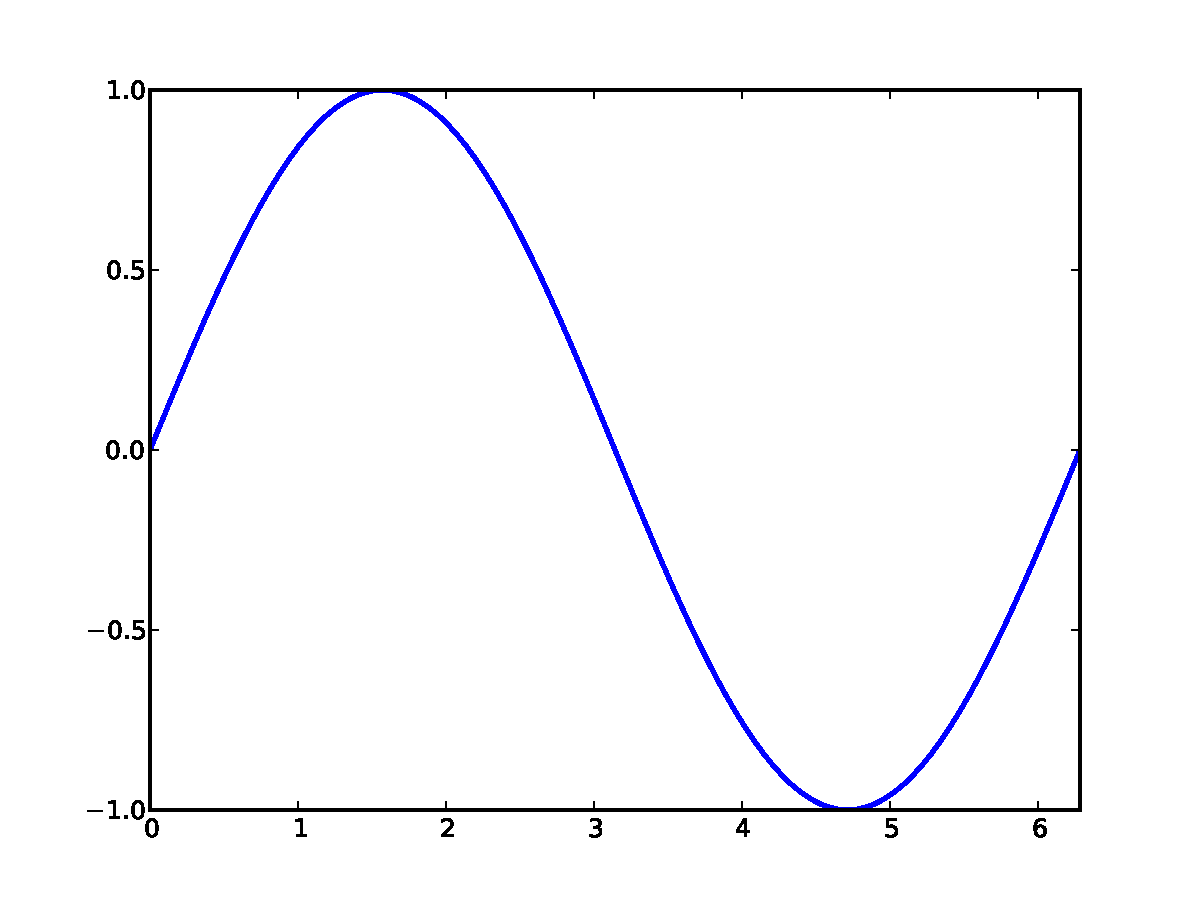
\includegraphics[width=.9\textwidth]{sine}
  \caption{Illustration of how to include a figure. }
  \label{fig:sine}
\end{figure}




%%%%%%%%%%%%%%%%%%%%%%%%%%%%%%%%%%%%%%%%%%%%%%%%%%
% Keep the following \cleardoublepage at the end of this file,
% otherwise \includeonly includes empty pages.
\cleardoublepage

% vim: tw=70 nocindent expandtab foldmethod=marker foldmarker={{{}{,}{}}}
